\documentclass{article}
\usepackage[utf8]{inputenc}
\usepackage{float}
\usepackage{listings}
\usepackage{enumitem}
\usepackage{todonotes}
\usepackage{pdflscape}
\usepackage[htt]{hyphenat}
\usepackage{minted}
\usepackage{makecell}

\title{MI-FME Cvičení 6}
\author{Tomáš Chvosta}
\date{Březen 2020}

\setcounter{secnumdepth}{-2} % no numbered sections
\usepackage{czech}
\begin{document}

\maketitle

\section{Zadání}

Stáhněte si soubor \texttt{search.riscal} z Moodlu. Tento soubor reprezentuje specifikaci vyhledávání řetězce v RISCAL. V této specifikaci jsou řetězce reprezentovány jako pole znaků, kde znaky reprezentují přirozená čísla (včetně nuly).

\begin{itemize}
				
	\item Spusťte soubor v RISCAL ( checkbox "Nondeterminism" by neměl být zaškrtnut a jako "Operation" zvolte \texttt{exec}(), poté klikněte na zelenou šipku v sekci "Analysis".
	
	\item Přečtěte si zdrojový kód souboru a pokuste se ho pochopit.
	
	\item Upravte zdrojový kód tak, aby výskyt čísla $0$ v řetezci $a$ byl interpretován jako žolíkový znak, tedy aby představoval kterýkoliv znak.
					
\end{itemize}

\section{Analýza}

Program obsahuje jeden predikát $atpos$ a jednu funkci $contains$. Predikát $atpos$ vypadá následovně:
$$((len\_s \leq N) \wedge (p+len\_a \leq len\_s) \wedge (\forall i \in index)(i < len\_a \Rightarrow (s[p+i]=a[i])))$$
Proměnná $s$ představuje řetězec délky $len\_s$, ve kterém se vyhledává, $a$ představuje hledaný řetězec délky $len\_a$. Funkce $contains$ vrací množinu indexů, které splňují predikát $atpos$. Jinými slovy tedy vrací indexy, na kterých se nachází hledaný řetězec $a$ v řetězci $s$.

\section{Řešení}

Původní řešení nabízelo vyhledávání a výpis výskytů řetězce $a$ v řetězci $s$. V predikátu $atpos$ je jasně definováno, že od indexu, který má být výsledkem se všechny znaky musí shodovat pro všechny indexi v řetězci $a$. Nám tedy stačí rozšířit část predikátu $s[p+i]=a[i]$ o možnost, kdy je $a[i] = 0 $. Pokud je totiž $a[i] = 0$, pak $s[p+i]$ může být kterýkoliv znak. Predikát tedy upravíme na následující tvar:
$$((len\_s \leq N) \wedge (p+len\_a \leq len\_s)$$ $$\wedge$$ $$(\forall i \in index)(i < len\_a \Rightarrow ((s[p+i]=a[i]) \ \lor \ (a[i]=0))))$$
Touto změnou dosáhneme požadovaného výsledku. Na následujícím obrázku je vidět upravený kód a také jeden z běhů programu.

\begin{figure}[H]
    \centering
    \caption{Ukázka programu search.riscal}
    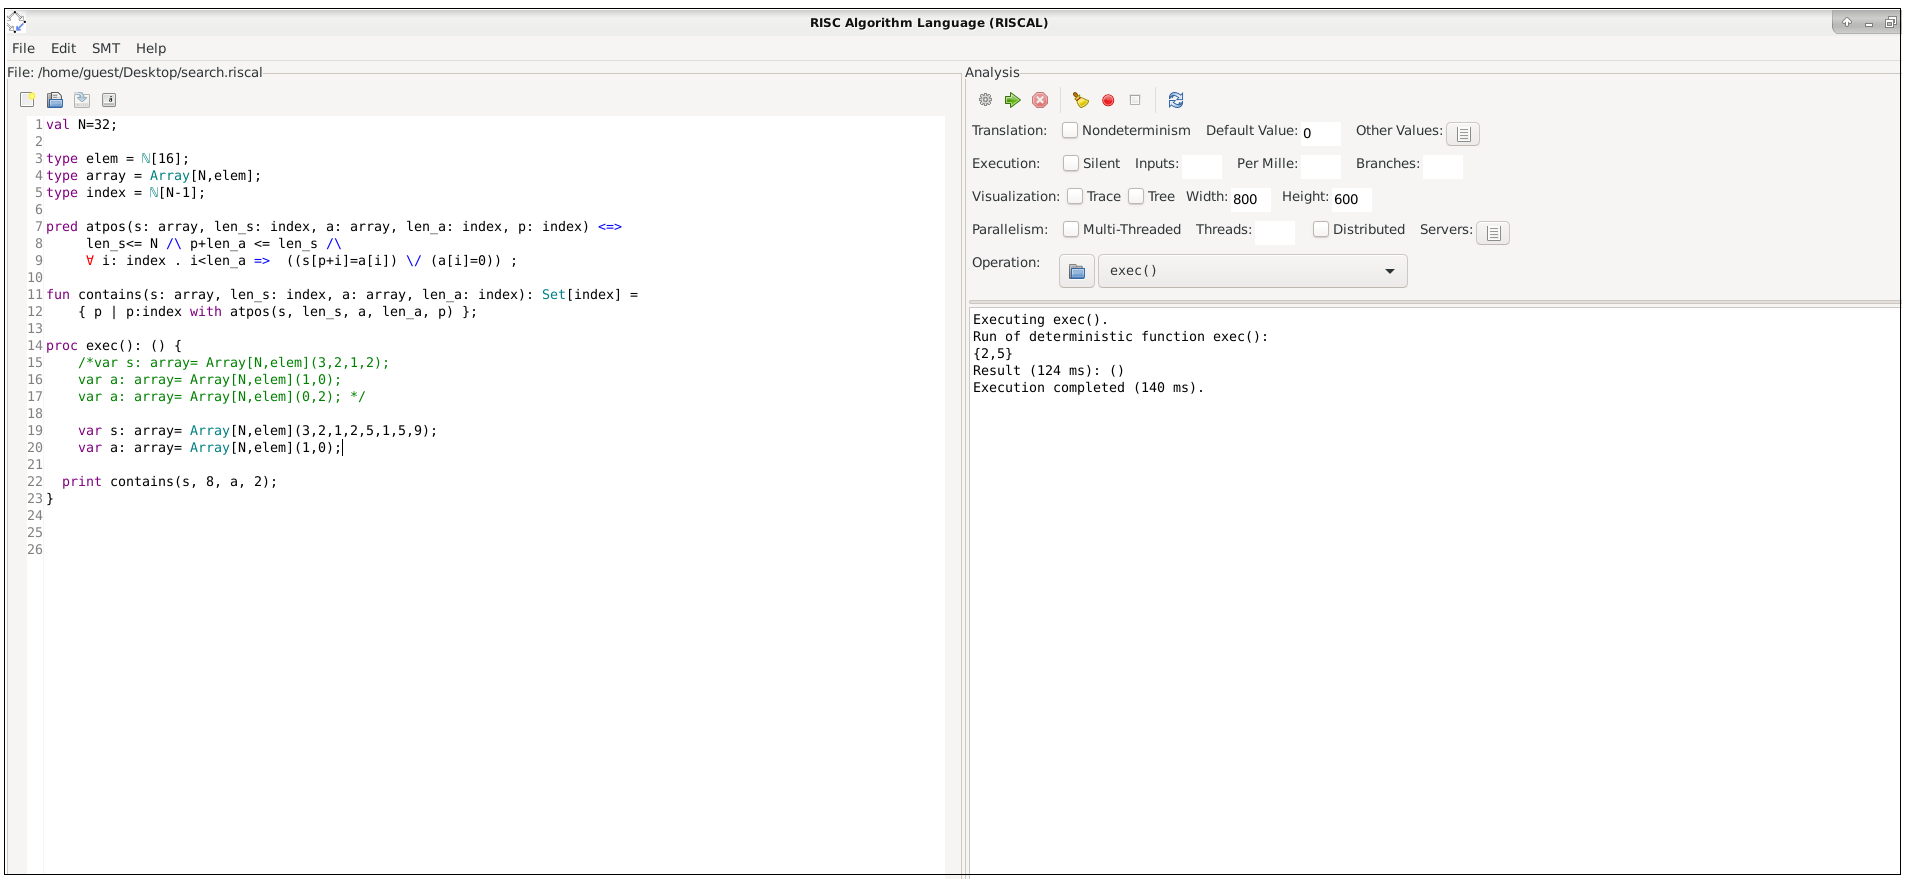
\includegraphics[width=\textwidth]{RiscalRun.png}
\end{figure}

\end{document}
